In this section, we will give informal intuition of our problem and then formally define it as a constraint satisfaction problem which is analogous to an orienteering problem.

\subsection{Problem Objective}

Our objective is to propose an optimization of university space based on a supply and demand analysis specific to staff meeting rooms and student toilet facilities. We are required to analyze the spatial data, employee data, timetabling data, and meetings held data to advise if the supply of meeting rooms and toilets on campus meets the current demand, and how the arrangement and maintenance services can be optimized accordingly.

Using the provided data, we performed the initial data analysis to get the basic idea of the supply-demand problem across campuses, buildings, and corresponding floors. To propose an optimization of current university space for using supply-demand effectively, we aimed at devising solutions that can efficiently use the current supply of the resources. Using this intuition, we transformed this general objective into a prediction problem that aims at predicting the best entity that can give the best supply of the resources based on demand and other preferences or factors. These prediction objectives enabled us to get a deeper insight into the data and can be informally stated as follows:

\begin{itemize}
    \item \textbf{Finding the $k$-best nearest buildings}: In this objective, we are aiming to find the $k$-best nearest buildings from a particular building that is having a good supply of meeting room or student toilet facilities based on factors like easy availability, excellent conditions, COVID-19 lockdown, etc.
    
    \item \textbf{Finding the $k$-best nearest floors}: In this objective, we are aiming to find the $k$-best nearest floors in a particular building based on supply and demand of meeting rooms and student toilet facilities. We also enabled the filtering of results based on factors like easy availability, excellent conditions, COVID-19 lockdown, etc.
\end{itemize}

These prediction-based objectives helped us to represent a general space optimization problem into more concrete strategy-based objectives. The above prediction objectives aim is to provide a critical understanding of the supply-demand that can help us to create strategies that will lead to the usage of the current supply of the resources more effectively. We will now formally represent these objectives in the below section.

\subsection{Problem Formulation} \label{formulation}

In this section, we will represent previously stated prediction objectives into a formal constraint satisfaction mathematical problem which can then be solved using our proposed non-randomized orienteering algorithm. Both of our objectives of finding the $k$-best nearest buildings and floors based on supply, demand, and factors can be formally described using the same problem as shown below.

The idea of our problem is to find the $k$-best optimal building or floor within a provided radius or provided number of floors which maximizes the reward of booking a meeting room or using a toilet facility based on different factors. We can define this idea by considering a traveling budget $B$, provided objective $O$, and a set of factors $F$. Here, $O \in $ \{\textit{book meeting room}, \textit{use toilet facility}\}, $F \in $ \{\textit{easy availability, room conditions, COVID-19 lockdown, ....} \} and $B \in \R_0^+ \cup \{\infty\}$. We will now formulate our domain-related optimal building finding problem into a generic orienteering problem (OP) for a specialized graph. We can represent our situation of finding $k$-the best optimal building or floor from a particular building or floor using a specialized graph as described below.

Let us assume a weighted directed specialized graph $G_s = (V,E)$ for $n$ number of nodes where $v_s \in V$ is the pre-defined start node such that,
\begin{gather}
     V = \{v_1, v_2, v_3,...,v_n\} \\
    E = \{(v_s, v_i)\:\backslash\:(v_s, v_s)\:|\:\forall\:i \in [1,n]\:\}
\end{gather}
Here, $v_s$ is having $n$ out-degree with 0 in-degree (i.e. $v_s$ is connected to every other node in $V$) and $v_i\:\forall\:i \in [1,n]$ \textbackslash $\:v_s$ is connected to only $v_s$ with 1 in-degree and 0 out-degree. 

Let $v_g$ be the set of $k$-optimal goal nodes s.t. $v_g \in V$ and $k \leq n$. These goals are attained in the decreasing order of their gained rewards after respecting budget constraints (i.e. $v_{g1} > v_{g2} > ... > v_{gk}$). 

Let $r$ be the set of nodes which we can visit such that $r \subseteq V$ \textbackslash\:$v_s$. 

% Let $B$ be the traveling budget which will enable the budget constraints. Let $O$ be the generic objectives and $F$ be the generic factors that can be used to tweak the reward function of the problem. 

For each $r$, let $R(r, o, f)$ be the reward function where $\:R:(r,o,f) \rightarrow {\rm I\!R}_0^+ \cup \{\infty\}$ calculates the reward based on the provided set of factors $f \subseteq F$ and objective $o \in O$. 

Let $I(r) = R(r,o,f)$ be the reward gained by visiting each node in $r$. 

Let the cost of traversal be given by $C(r) = C(v_s, v_i^r)$, where $v_i$ is the $i^{th}$ element in $r$, $\forall i \in [1,|r|]$. 

Let $L \in {\rm I\!R}_0^+ \cup \{\infty\}$ be the constraint limit. 

Using the above notations, the hard-constraint problem can then be defined by the equation \ref{eq_3}.
\begin{equation} \label{eq_3}
    \argmax_{r \subseteq V}I(r) \:\textit{subject to}\:C(r) \leq B \leq L
\end{equation}

We can relax the above hard-constraint by introducing a hyper-parameter $\delta$ to formulate a soft-constraint problem as shown in the equation \ref{eq_4}.
\begin{equation} \label{eq_4}
    \argmax_{r \subseteq V}I(r) \:\textit{subject to}\: C(r) \leq B+\delta \leq L
\end{equation}

where $\delta \in {\rm I\!R}_0^+ \cup \{\infty\}$.

Informally, the solution to our stated problem is a set of ordered $k$-optimal goal nodes, such that the reward obtained by visiting the node is maximized while the path cost stays within a specified traveling budget $B$.

\subsubsection{Example: Applying formulation for finding 3-best nearest buildings} \label{example_1}

In this section, we will use the above formulation to implement an example problem of finding the 3-best nearest building for booking a meeting room from building 220 (780 Elizabeth St) in the Parkville campus. We will first generate a specialized graph of all the buildings, as described in the above formulation, from building 220 where a snapshot of the example graph is shown below.

\begin{figure}[H]
\centering
  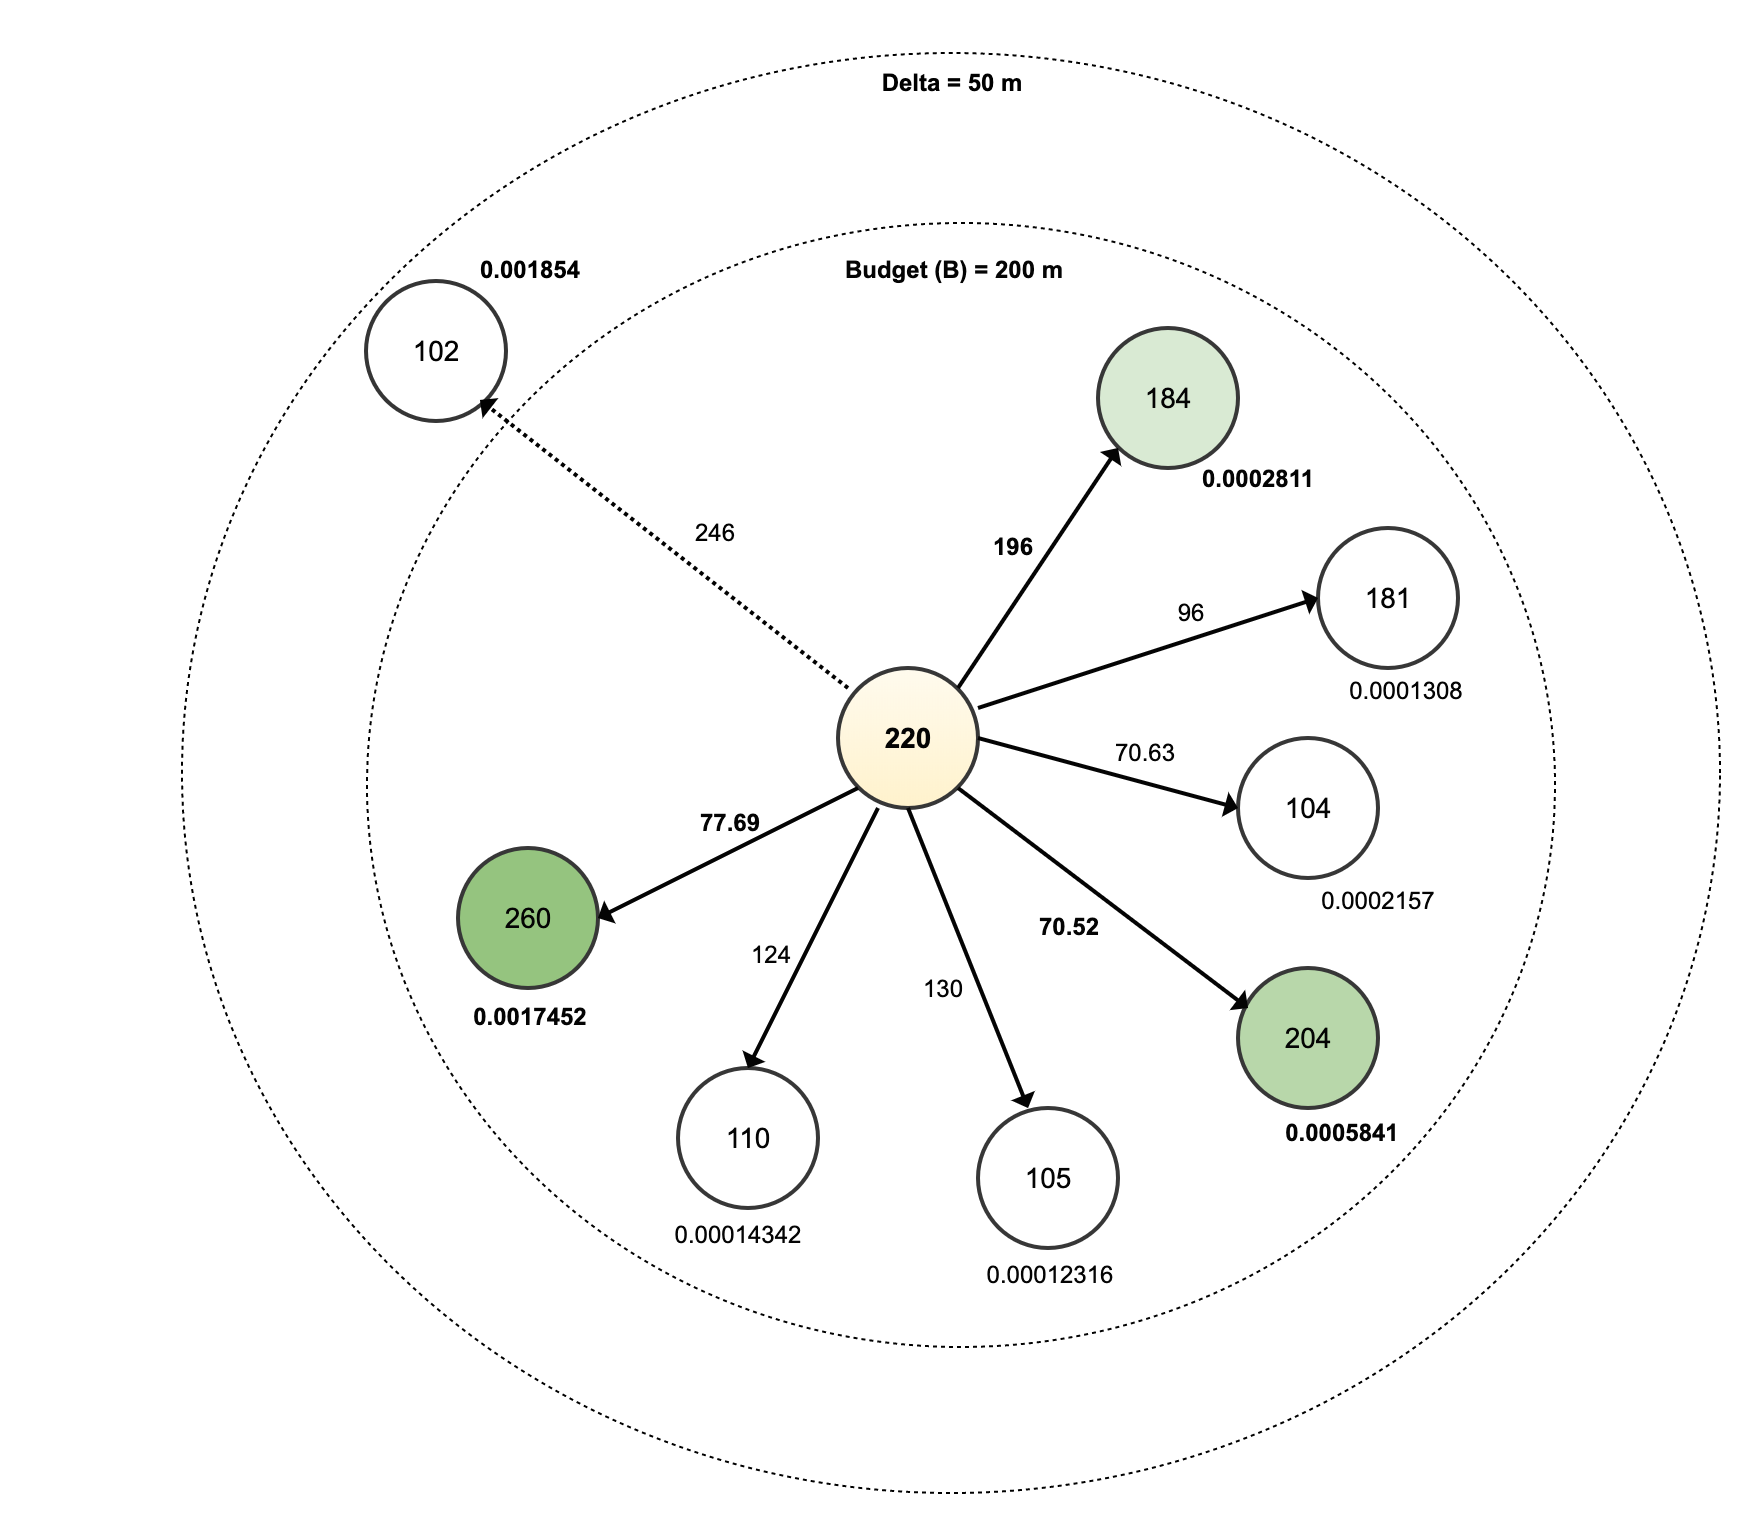
\includegraphics[width=8cm,keepaspectratio=true]{csp.png}
  \label{fig:cop}
  \caption{Specialized graph from Building 220 to all nearby buildings with their corresponding rewards}
\end{figure}

Now, as per our above graph, we have Budget $B = 200$ metres, $o = \textit\{{book\:meeting\:room}\}\in O$, and $F \in $ \{\textit{easy availability, COVID lockdown, ....} \}. Let $V_c =\{220, 184,181,104,204,105,110,260,102\}$  be the set of $10$ buildings in a campus $c = PARKVILLE$. Let $v_s = 220$ be the starting building such that $v_s \in V_c$. Let $r = \{184,181,104,204,105,110,260,102\}$ be the set of buildings a person can visit s.t. $r \subseteq V_c$ \textbackslash\:$v_s$. For each $r$, the reward gained $I(r) = R(r,o,f)$ by visiting each building in $r$, for provided objective $o \in O$ and factors $f \in F$ can be stated as shown using below table with respective cost $C(r)$.

\begin{table}[H]
\centering
\begin{tabular}{|l|l|l|l|l|}
\hline
$r \subseteq V_c$ \textbackslash\:$v_s$   & $o \in O$                  & $f \in F$ & $I(r) = R(r,o,f)$ & $C(r) = C(220, v_i^r)$ \\ \hline
184 & \textit{book meeting room} & $\emptyset$  & 0.0002811 & 196     \\ \hline
181 & \textit{book meeting room} & $\emptyset$                     & 0.0001308 & 96     \\ \hline
104 & \textit{book meeting room} & $\emptyset$                        & 0.0002157 & 70.63    \\ \hline
204 & \textit{book meeting room} & $\emptyset$                    & 0.0005841  & 70.52   \\ \hline
105 & \textit{book meeting room} & $\emptyset$                          & 0.00012316 & 130    \\ \hline
110 & \textit{book meeting room} & $\emptyset$                          & 0.00014342 & 124    \\ \hline
260 & \textit{book meeting room} & $\emptyset$                          & 0.0017452  & 77.69   \\ \hline
102 & \textit{book meeting room} & $\emptyset$                         & 0.001854 & 246    \\ \hline
\end{tabular}
\caption{Example problem cost-reward table for finding 3-best nearest buildings}
 \label{tab:cost_reward_1}
\end{table}

Now, we need to find the set of goal building $v_g$ s.t. $v_g \in V_c$ and satisfies below hard constraint.
\begin{equation}
    \argmax_{r \subseteq V_c}I(r) \:\textit{subject to}\:C(r) \leq B=200
\end{equation}
Similarly, we can also find the set of goal building $v_g*$ s.t. $v_g* \in V_c$ and satisfies below soft constraint.
\begin{gather}
     \argmax_{r \subseteq V_c}I(r) \:\textit{subject to}\: C(r) \leq B+\delta = 200+50 = 250
\end{gather}

where $\delta = 50 \in \R_0^+ \cup \{\infty\}$.

We will solve these equations using our proposed non-randomized orienteering algorithm as discussed in the section \ref{methodologies}.

% \subsubsection{Example: Applying formulation for finding 3-best nearest floors} \label{example_2}

% In this section, we will again use the above formulation to implement an example problem of finding the 3-best nearest floors for booking a meeting room from Level 2 of Redmond Berry Building in the Parkville campus. We will first generate a specialized graph of all the floors, as described in the above formulation, from Level 2 where a snapshot of the example graph is shown below.
% \vspace{-2mm}
% \begin{figure}[H]
% \centering
%   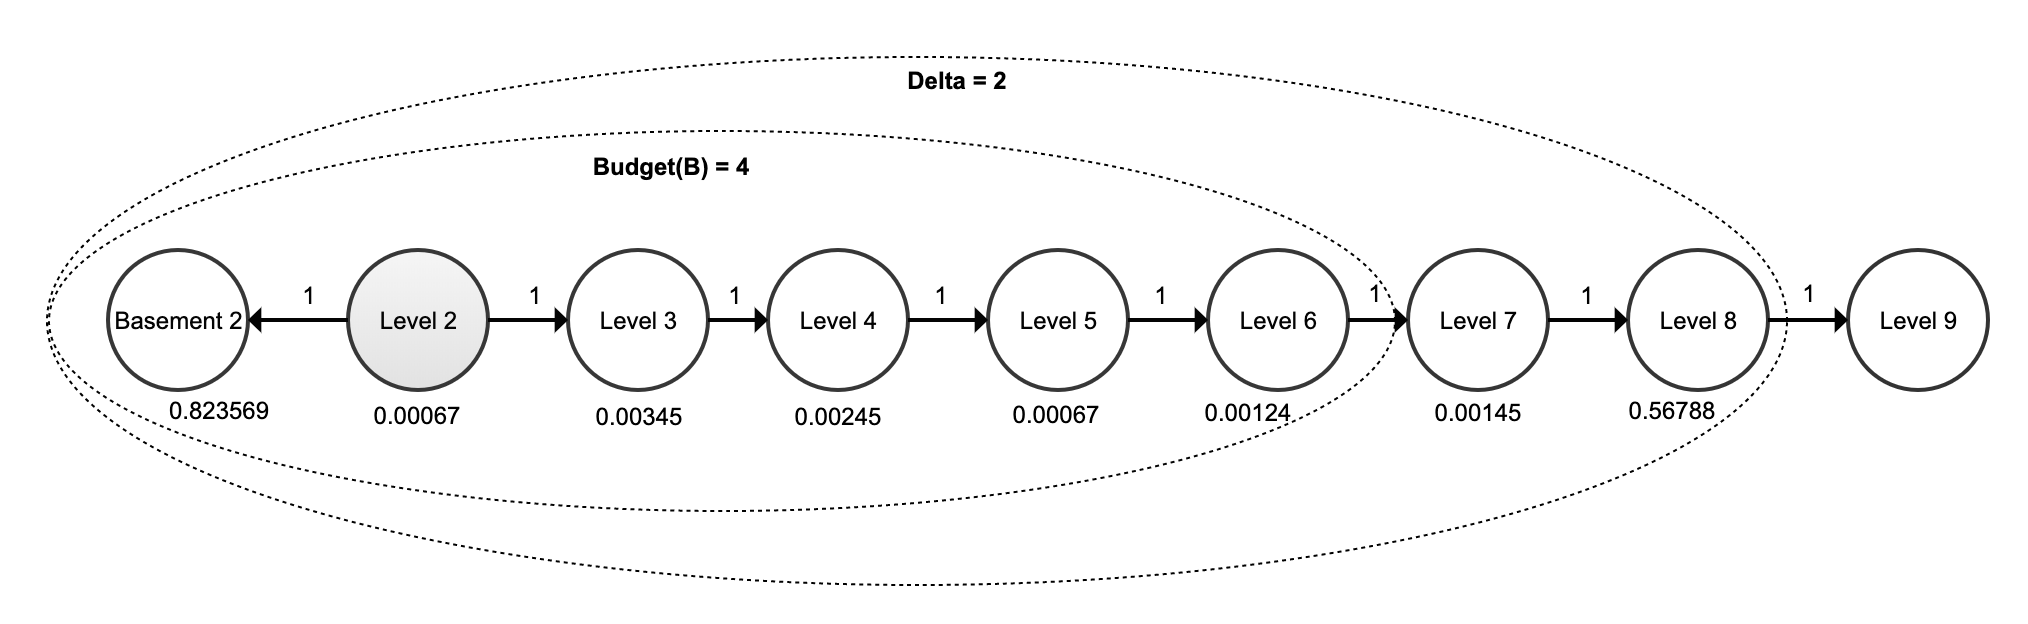
\includegraphics[width=12cm,keepaspectratio=true]{csp_floor.png}
%   \label{fig:csp_floor}
%   \caption{Specialized graph from Level 2 to all other floors with their corresponding rewards}
% \end{figure}
% \vspace{-4mm}
% Now, as per our above graph, we have Budget $B = 4$, $o = \{\textit{book meeting room}\} \in O$, and $F \in $ \{\textit{easy availability, COVID lockdown, ....} \}. Let $V_b =\{$\textit{Basement 2, Level 2, Level 3, Level 4, Level 5, Level 6, Level 7, Level 8, Level 9}$\}$  be the set of $10$ floors in a building $b = $\textit{Redmond barry building}. Let $v_s = $ \textit{Level 2} be the starting floor of building $b$ such that $v_s \in V_b$. Let $r = \{$\textit{Basement 2, Level 3, Level 4, Level 5, Level 6, Level 7, Level 8, Level 9}$\}$ be the set of floors a person can visit s.t. $r \subseteq V_b$ \textbackslash\:$v_s$. For each $r$, the reward gained $I(r) = R(r,o,f)$ by visiting each building in $r$, for provided objective $o \in O$ and factors $f \in F$ can be stated as shown using below table with respective cost $C(r)$.

% \begin{table}[H]
% \centering
% \begin{tabular}{|l|l|l|l|l|}
% \hline
% $r \subseteq V_c$ \textbackslash\:$v_s$   & $o \in O$                  & $f \in F$ & $I(r) = R(r,o,f)$ & $C(r) = C(L2, v_i^r)$ \\ \hline
% \textit{Basement 2} & \textit{book meeting room} & $\emptyset$  & 0.823569 & 1     \\ \hline
% \textit{Level 3} & \textit{book meeting room} & $\emptyset$                        & 0.00345 & 1     \\ \hline
% \textit{Level 4} & \textit{book meeting room} & $\emptyset$                          & 0.00245 & 2    \\ \hline
% \textit{Level 5} & \textit{book meeting room} & $\emptyset$                     & 0.00067  & 3  \\ \hline
% \textit{Level 6} & \textit{book meeting room} & $\emptyset$                          & 0.00124 & 4    \\ \hline
% \textit{Level 7} & \textit{book meeting room} & $\emptyset$                          & 0.00145 & 5    \\ \hline
% \textit{Level 8} & \textit{book meeting room} & $\emptyset$                          & 0.56788  & 6   \\ \hline
% \textit{Level 9} & \textit{book meeting room} & $\emptyset$                          & 0.00125 & 7    \\ \hline
% \end{tabular}
% \caption{Example problem cost-reward table for finding 3-best nearest floors}
%  \label{tab:cost_reward_2}
% \end{table}

% Now, we can find the set of goal floors $v_g$ s.t. $v_g \in V_c$ that satisfies below hard constraint.
% \begin{equation}
%     \argmax_{r \subseteq V_c}I(r) \:\textit{subject to}\:C(r) \leq B=4 \leq Floors(b)
% \end{equation}
% Similarly, we can also find the set of goal floors $v_g*$ s.t. $v_g* \in V_c$ that satisfies below soft constraint.
% \begin{equation}
%      \argmax_{r \subseteq V_c}I(r) \:\textit{subject to}\: C(r) \leq B+\delta = 4+2 = 6 \leq Floors(b) = L
% \end{equation}

% where $\delta = 2 \in \R_0^+ \cup \{\infty\} \leq L-B$

% We will again solve these equations using our proposed non-randomized orienteering algorithm as discussed in the section\ref{solution}.